\documentclass{standalone}
\usepackage{tikz}
\usetikzlibrary{patterns, positioning}

\begin{document}
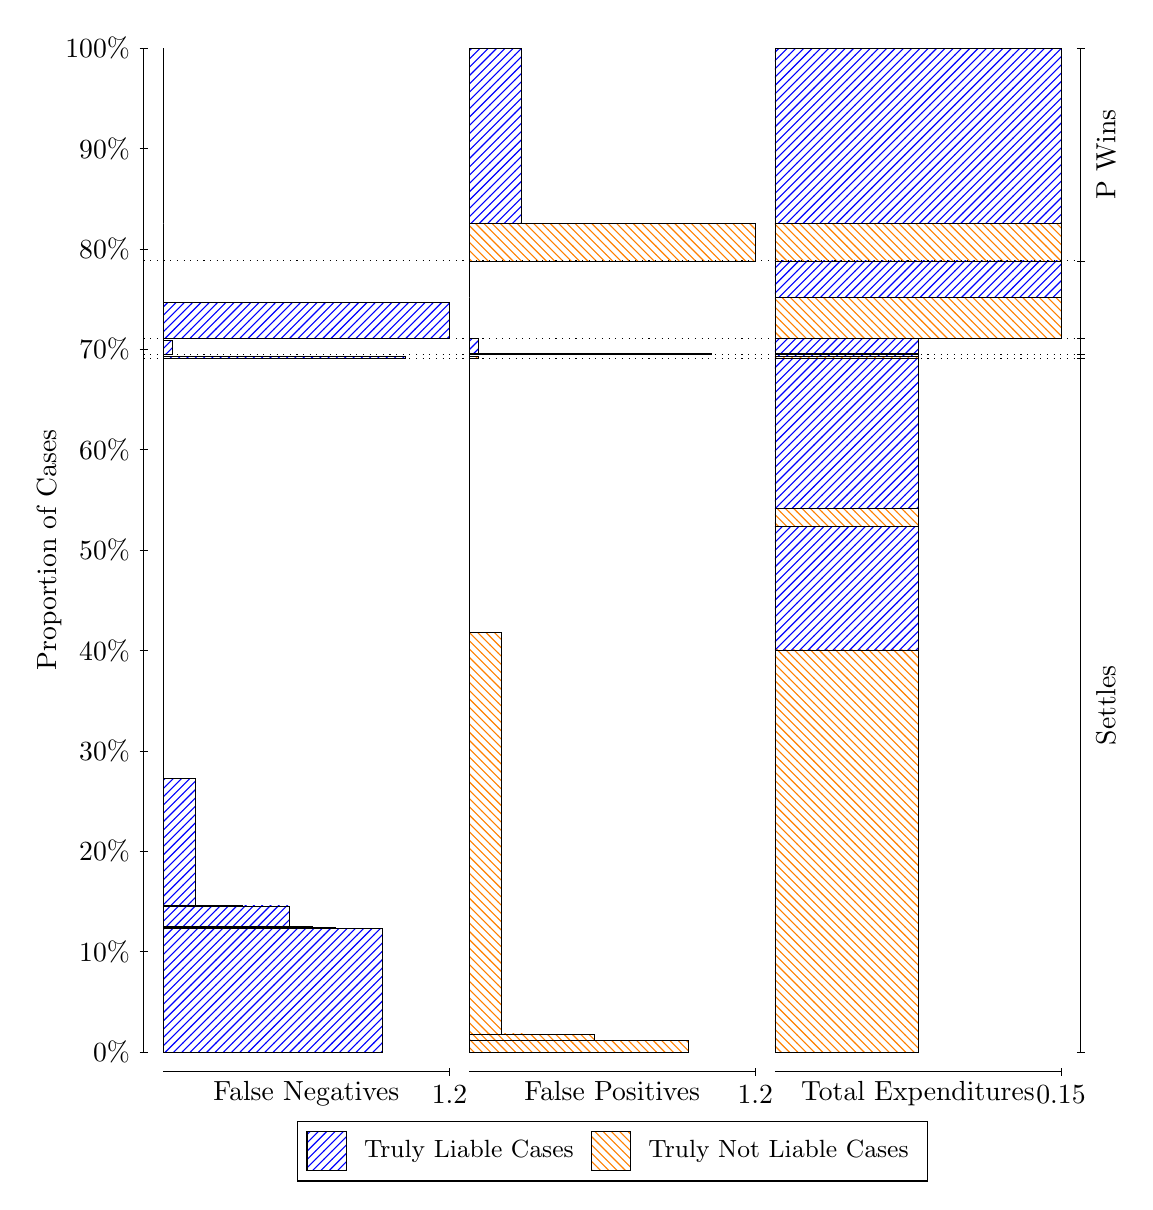
\begin{tikzpicture}
\draw[black, very thin] (1.5,1.75) -- (1.5,14.5);
\node[rotate=90, anchor=center] at (0.3, 8.125) {Proportion of Cases};
\draw[black, very thin] (1.45,1.75) -- (1.55,1.75);
\node[anchor=east] at (1.45, 1.75) {0\%};
\draw[black, very thin] (1.45,3.025) -- (1.55,3.025);
\node[anchor=east] at (1.45, 3.025) {10\%};
\draw[black, very thin] (1.45,4.3) -- (1.55,4.3);
\node[anchor=east] at (1.45, 4.3) {20\%};
\draw[black, very thin] (1.45,5.575) -- (1.55,5.575);
\node[anchor=east] at (1.45, 5.575) {30\%};
\draw[black, very thin] (1.45,6.85) -- (1.55,6.85);
\node[anchor=east] at (1.45, 6.85) {40\%};
\draw[black, very thin] (1.45,8.125) -- (1.55,8.125);
\node[anchor=east] at (1.45, 8.125) {50\%};
\draw[black, very thin] (1.45,9.4) -- (1.55,9.4);
\node[anchor=east] at (1.45, 9.4) {60\%};
\draw[black, very thin] (1.45,10.675) -- (1.55,10.675);
\node[anchor=east] at (1.45, 10.675) {70\%};
\draw[black, very thin] (1.45,11.95) -- (1.55,11.95);
\node[anchor=east] at (1.45, 11.95) {80\%};
\draw[black, very thin] (1.45,13.225) -- (1.55,13.225);
\node[anchor=east] at (1.45, 13.225) {90\%};
\draw[black, very thin] (1.45,14.5) -- (1.55,14.5);
\node[anchor=east] at (1.45, 14.5) {100\%};

\draw[black, very thin] (13.4,1.75) -- (13.4,14.5);
\draw[black, very thin] (13.35,1.75) -- (13.45,1.75);
\node[anchor=west] at (13.35, 1.75) {};
\draw[black, very thin] (13.35,10.559) -- (13.45,10.559);
\node[anchor=west] at (13.35, 10.559) {};
\draw[black, very thin] (13.35,10.608) -- (13.45,10.608);
\node[anchor=west] at (13.35, 10.608) {};
\draw[black, very thin] (13.35,10.808) -- (13.45,10.808);
\node[anchor=west] at (13.35, 10.808) {};
\draw[black, very thin] (13.35,11.798) -- (13.45,11.798);
\node[anchor=west] at (13.35, 11.798) {};
\draw[black, very thin] (13.35,14.5) -- (13.45,14.5);
\node[anchor=west] at (13.35, 14.5) {};

\draw[black, very thin, pattern color=blue, pattern=north east lines] (1.75,1.75) rectangle (4.5306,3.3155);
\draw[black, very thin, pattern color=blue, pattern=north east lines] (1.75,3.3155) rectangle (4.234,3.3236);
\draw[black, very thin, pattern color=blue, pattern=north east lines] (1.75,3.3236) rectangle (3.9374,3.332);
\draw[black, very thin, pattern color=blue, pattern=north east lines] (1.75,3.332) rectangle (3.6408,3.3406);
\draw[black, very thin, pattern color=blue, pattern=north east lines] (1.75,3.3406) rectangle (3.3442,3.6041);
\draw[black, very thin, pattern color=blue, pattern=north east lines] (1.75,3.6041) rectangle (3.0476,3.6056);
\draw[black, very thin, pattern color=blue, pattern=north east lines] (1.75,3.6056) rectangle (2.751,3.6071);
\draw[black, very thin, pattern color=blue, pattern=north east lines] (1.75,3.6071) rectangle (2.4544,3.6085);
\draw[black, very thin, pattern color=blue, pattern=north east lines] (1.75,3.6085) rectangle (2.1578,5.2269);
\draw[black, very thin, pattern color=orange, pattern=north west lines] (1.75,5.2269) rectangle (1.75,10.559);
\draw[black, very thin, pattern color=blue, pattern=north east lines] (1.75,10.559) rectangle (4.8272,10.581);
\draw[black, very thin, pattern color=orange, pattern=north west lines] (1.75,10.581) rectangle (1.75,10.608);
\draw[black, very thin, pattern color=blue, pattern=north east lines] (1.75,10.608) rectangle (1.8612,10.79);
\draw[black, very thin, pattern color=orange, pattern=north west lines] (1.75,10.79) rectangle (1.75,10.808);
\draw[black, very thin, pattern color=blue, pattern=north east lines] (1.75,10.808) rectangle (5.3833,11.273);
\draw[black, very thin, pattern color=orange, pattern=north west lines] (1.75,11.273) rectangle (1.75,11.798);
\draw[black, very thin, pattern color=orange, pattern=north west lines] (1.75,11.798) rectangle (1.75,12.271);
\draw[black, very thin, pattern color=blue, pattern=north east lines] (1.75,12.271) rectangle (1.75,14.5);
\draw[black, very thin, pattern color=orange, pattern=north west lines] (5.6333,1.75) rectangle (8.4139,1.8957);
\draw[black, very thin, pattern color=orange, pattern=north west lines] (5.6333,1.8957) rectangle (8.1173,1.896);
\draw[black, very thin, pattern color=orange, pattern=north west lines] (5.6333,1.896) rectangle (7.8207,1.8963);
\draw[black, very thin, pattern color=orange, pattern=north west lines] (5.6333,1.8963) rectangle (7.5241,1.8966);
\draw[black, very thin, pattern color=orange, pattern=north west lines] (5.6333,1.8966) rectangle (7.2276,1.9718);
\draw[black, very thin, pattern color=orange, pattern=north west lines] (5.6333,1.9718) rectangle (6.931,1.9718);
\draw[black, very thin, pattern color=orange, pattern=north west lines] (5.6333,1.9718) rectangle (6.931,1.9743);
\draw[black, very thin, pattern color=orange, pattern=north west lines] (5.6333,1.9743) rectangle (6.6344,1.9766);
\draw[black, very thin, pattern color=orange, pattern=north west lines] (5.6333,1.9766) rectangle (6.3378,1.979);
\draw[black, very thin, pattern color=orange, pattern=north west lines] (5.6333,1.979) rectangle (6.0412,7.0821);
\draw[black, very thin, pattern color=blue, pattern=north east lines] (5.6333,7.0821) rectangle (5.6333,10.559);
\draw[black, very thin, pattern color=orange, pattern=north west lines] (5.6333,10.559) rectangle (5.7446,10.586);
\draw[black, very thin, pattern color=blue, pattern=north east lines] (5.6333,10.586) rectangle (5.6333,10.608);
\draw[black, very thin, pattern color=orange, pattern=north west lines] (5.6333,10.608) rectangle (8.7105,10.626);
\draw[black, very thin, pattern color=blue, pattern=north east lines] (5.6333,10.626) rectangle (5.7446,10.808);
\draw[black, very thin, pattern color=orange, pattern=north west lines] (5.6333,10.808) rectangle (5.6333,11.333);
\draw[black, very thin, pattern color=blue, pattern=north east lines] (5.6333,11.333) rectangle (5.6333,11.798);
\draw[black, very thin, pattern color=orange, pattern=north west lines] (5.6333,11.798) rectangle (9.2667,12.271);
\draw[black, very thin, pattern color=blue, pattern=north east lines] (5.6333,12.271) rectangle (6.3007,14.5);
\draw[black, very thin, pattern color=orange, pattern=north west lines] (9.5167,1.75) rectangle (11.333,6.8554);
\draw[black, very thin, pattern color=blue, pattern=north east lines] (9.5167,6.8554) rectangle (11.333,8.4291);
\draw[black, very thin, pattern color=orange, pattern=north west lines] (9.5167,8.4291) rectangle (11.333,8.6557);
\draw[black, very thin, pattern color=blue, pattern=north east lines] (9.5167,8.6557) rectangle (11.333,10.559);
\draw[black, very thin, pattern color=orange, pattern=north west lines] (9.5167,10.559) rectangle (11.333,10.586);
\draw[black, very thin, pattern color=blue, pattern=north east lines] (9.5167,10.586) rectangle (11.333,10.608);
\draw[black, very thin, pattern color=orange, pattern=north west lines] (9.5167,10.608) rectangle (11.333,10.626);
\draw[black, very thin, pattern color=blue, pattern=north east lines] (9.5167,10.626) rectangle (11.333,10.808);
\draw[black, very thin, pattern color=orange, pattern=north west lines] (9.5167,10.808) rectangle (13.15,11.333);
\draw[black, very thin, pattern color=blue, pattern=north east lines] (9.5167,11.333) rectangle (13.15,11.798);
\draw[black, very thin, pattern color=orange, pattern=north west lines] (9.5167,11.798) rectangle (13.15,12.271);
\draw[black, very thin, pattern color=blue, pattern=north east lines] (9.5167,12.271) rectangle (13.15,14.5);
\draw[black, dotted] (1.5,10.559) -- (13.4,10.559);
\draw[black, dotted] (1.5,10.608) -- (13.4,10.608);
\draw[black, dotted] (1.5,10.808) -- (13.4,10.808);
\draw[black, dotted] (1.5,11.798) -- (13.4,11.798);
\draw[black, very thin] (1.75,1.5) -- (5.3833,1.5);
\node[anchor=north] at (3.5667, 1.5) {False Negatives};
\draw[black, very thin] (5.3833,1.45) -- (5.3833,1.55);
\node[anchor=north] at (5.3833, 1.45) {1.2};

\draw[black, very thin] (5.6333,1.5) -- (9.2667,1.5);
\node[anchor=north] at (7.45, 1.5) {False Positives};
\draw[black, very thin] (9.2667,1.45) -- (9.2667,1.55);
\node[anchor=north] at (9.2667, 1.45) {1.2};

\draw[black, very thin] (9.5167,1.5) -- (13.15,1.5);
\node[anchor=north] at (11.333, 1.5) {Total Expenditures};
\draw[black, very thin] (13.15,1.45) -- (13.15,1.55);
\node[anchor=north] at (13.15, 1.45) {0.15};

\node[black, centered, rotate=90] at (13.72, 6.1545) {Settles};



\node[black, centered, rotate=90] at (13.72, 13.149) {P Wins};

\draw (7.449999999999999,1.5) node[draw=none] (baseCoordinate) {};
\begin{scope}[align=center]
        \matrix[scale=0.5, draw=black, below=0.5cm of baseCoordinate, nodes={draw}, column sep=0.1cm]{
            \node[rectangle, draw, minimum width=0.5cm, minimum height=0.5cm, pattern=north east lines, pattern color=blue] {}; &
            \node[draw=none, font=\small] (B) {Truly Liable Cases}; &
            \node[rectangle, draw, minimum width=0.5cm, minimum height=0.5cm, pattern=north west lines, pattern color=orange] {}; &
            \node[draw=none, font=\small] (B) {Truly Not Liable Cases}; \\
            };
\end{scope}

\end{tikzpicture}
\end{document}